%%%%%%%%%%%%%%%%%%%%%%%%%%%%%%%%%%%%%%%%%%%%%%%%%%%%%%%%%%%%%%%%%%%%%%%%%%%%%%%%%%
%%% Introduction
%%%%%%%%%%%%%%%%%%%%%%%%%%%%%%%%%%%%%%%%%%%%%%%%%%%%%%%%%%%%%%%%%%%%%%%%%%%%%%%%%%
\chapter{Introduction}

	\begin{figure}[h!]
		\centering
		\fbox{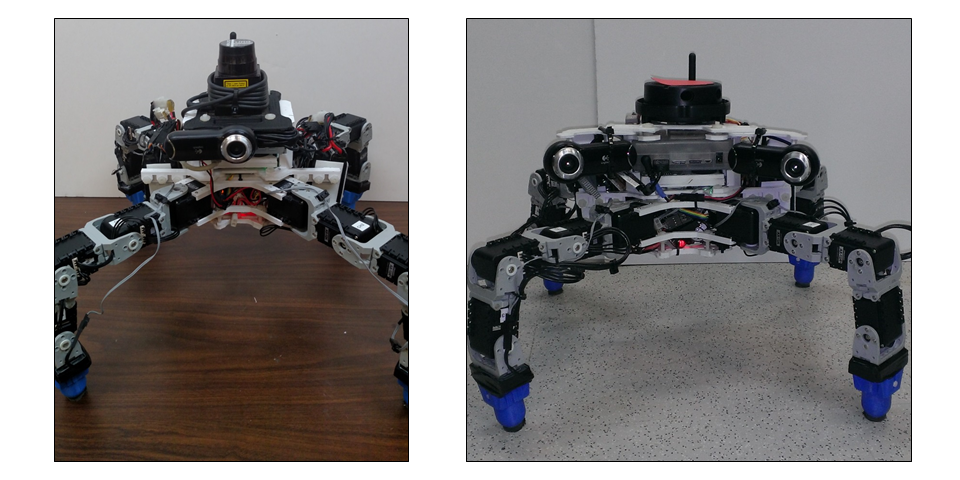
\includegraphics[width=\textwidth]{robot_selfies.png}}
		\caption{The BlueFoot Quadruped Robot: single-camera configuration \emph{(left)}; stereo-camera configuration \emph{(right)}}
		\label{fig::bluefoot}
	\end{figure}

		The design of legged robots and associated methods of locomotion control has been an area of interest spanning the past several decades, as shown by		
		\cite{
		McGhee1965,
		Hodgins1991, 
		Altendorfer2001, 
		Kolter2008
		}.
		Quadruped robotic systems have gained popularity in studies pertaining to variable terrain navigation and full-body stability adaptation. Well known examples of this from the past decade are the Tekken \cite{Fukuoka2003}, Kolt \cite{Estremera2006}, BigDog \cite{BigDog2008}, and HyQ \cite{Semini2010_PHD} quadrupeds. Many of these systems have been implemented on a larger scale so that they can carry substantial payloads while maintaining adequate system bandwidth for fast gaits and robustness to rough terrains. Few, however, have been implemented on the scale of a hobby-robot platform while still maintaining an aptitude for rough terrain navigation and comparable sensory prowess.

		The BlueFoot quadruped is a self-contained, fully-actuated platform with the dexterity to perform stabilization and  repositioning maneuvers on variable terrains along the same lines as the LittleDog platform \cite{Rebula2007}. BlueFoot includes a sizable array of on-board sensors for feedback and control. Using the computational capacities at hand, BlueFoot has the ability to utilize similar control mechanisms to those implemented on larger quadruped systems. BlueFoot is  gaited via a central pattern generator (CPG) based gaiting algorithm augmented with a foothold controller along the same lines as \cite{Ajallooeian2013} and \cite{Rutishauser2008}. Additionally, active platform stabilization is performed via a zero-moment point (ZMP) based body-posture controller which actively stabilizes the system during arbitrary gaiting sequences. The controllers presented in this paper make use of virtual-forces to drive system reference commands. An outer-loop controller supplies commands and corrections used in system navigation control.

**Not complete**